% -*- coding: utf-8 -*-
\documentclass[xetex,mathserif,serif]{beamer}

\usetheme{Berlin}
\usecolortheme{whale}

\usepackage{fontspec}
\usepackage{xunicode}
\usepackage{xltxtra}
\setmainfont[Mapping=tex-text]{GFS Bodoni}
\usepackage{xgreek}
\usepackage{graphicx}

\title[UFund] % (optional, only for long titles)
{UFund}
\subtitle{Συμμετοχική Πλατφόρμα Επενδύσεων}
\author % (optional, for multiple authors)
{Ν.~Βλασσόπουλος \and Γ.~Παπαγεωργίου}
\institute{}
\date[24-04-2016] % (optional)
{Hackathon @Innovathens}
%%\subject{Computer Science}

\begin{document}

\frame{\titlepage}

\begin{frame}
  \frametitle{Τί είναι το UFund;}
  \begin{itemize}
  \item Συμετοχική Πλατφόρμα Επενδύσεων
    \begin{itemize}
    \item Risk Sharing
    \item Micro-investments
    \item One-click investment
    \end{itemize}
  \item Gamificated Investment
  \end{itemize}
\end{frame}


\begin{frame}
  \frametitle{Flow}
  \begin{figure}
    \centering
    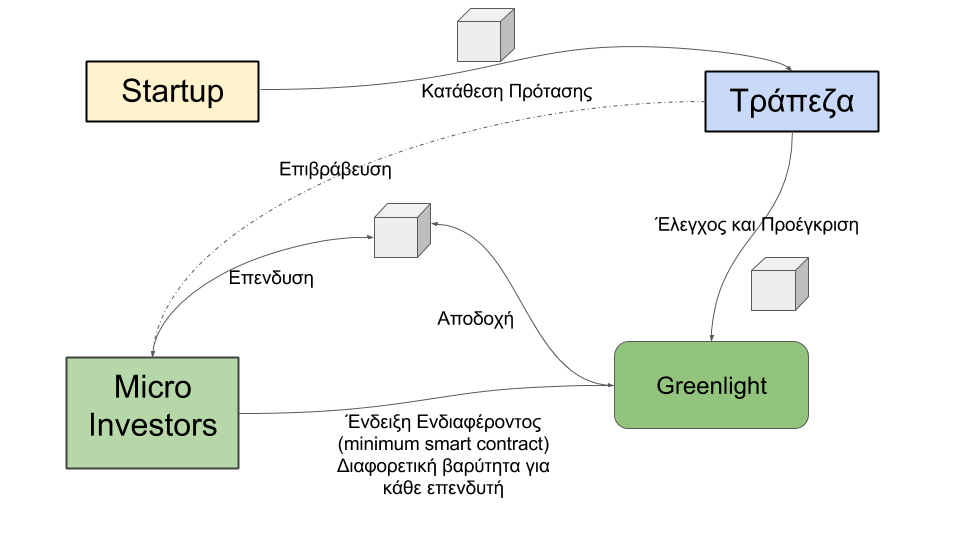
\includegraphics[width=0.85\textwidth]{hack-slide.png}
  \end{figure}
\end{frame}


\begin{frame}
  \frametitle{Τί επιτυγχάνει;}
  \framesubtitle{Τρείς διαφορετικοί ρόλοι...}

\begin{itemize}
\item Μικρο-επενδυτές
  \begin{itemize}
  \item Απαλλαγή από το ``τεχνικό'' κομμάτι της Επένδυσης (Evaluation, risk, etc)
  \item Επιβράβευση της επενδυτικής δραστηριότητας απο την Τράπεζα
  \item Συμμετοχή στην αναπτυξιακή προσπάθεια
  \end{itemize}

\item Τράπεζες
  \begin{itemize}
  \item Risk Sharing
  \item Feedback from investors
  \item A second level of ``security'' in the form of a ``Greenlight''
    process
  \item Συμμετοχή στην αναπτυξιακή προσπάθεια
  \end{itemize}
    
\item Startup
  \begin{itemize}
  \item Αμεσότερη χρηματοδότηση
  \end{itemize}
\end{itemize}
  
\end{frame}


\begin{frame}
  \frametitle{Tech Stack}
  \begin{figure}
    \centering
    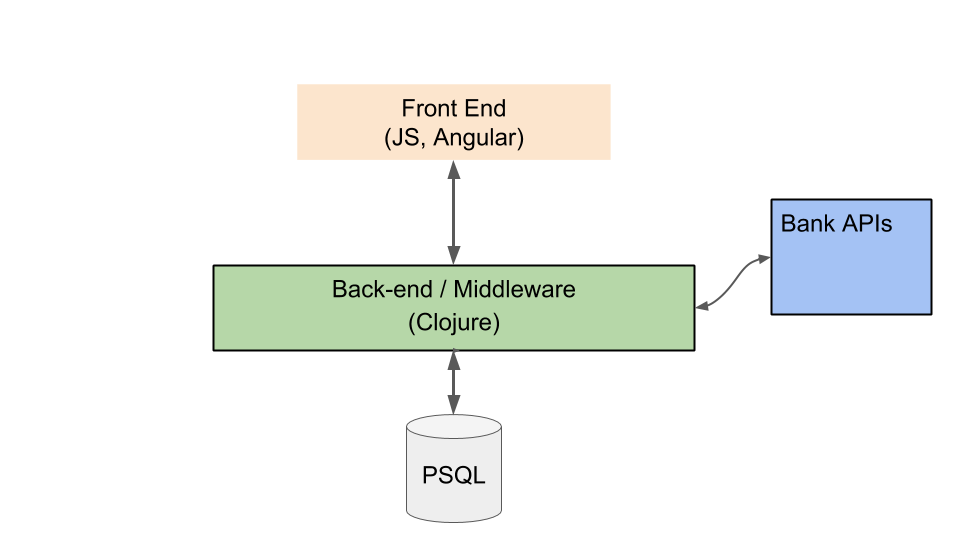
\includegraphics[width=0.85\textwidth]{hack-techflow.png}
  \end{figure}
\end{frame}


% etc
\end{document}


